\section{Maximum Matching in Bipartite Graphs} \label{sec_matching}
\noindent
%\vspace*{-1ex} %%! DO NOT USE HERE!!
%
%Here we begin with a wikipedia-like description of the maximum matching problem
% %including a few examples of important applications.
%
Given a graph $G=(V,E)$, a matching M in G is a set of pairwise non-adjacent edges.
%, none of which are loops; that is, no two edges share common vertices. A vertex is matched (or saturated) if it is an endpoint of one of the edges in the matching. Otherwise the vertex is unmatched. 
A maximum matching, also known as maximum-cardinality matching,
is a matching that contains the largest possible number of edges. 
Every maximum matching is maximal, but not every maximal matching 
is a maximum matching.

Versions of maximum matching problems arise in a number of contexts
and applications:
from flow and neural networks, scheduling and planning, modeling bonds 
in chemistry, graph coloring, the stable marriage problem, 
to matching kidney donors to kidney donor recipients, etc.

The 59-page chapter on maximum-flow problem formulations 
in~\cite{OPUS-book_algs-1990-MCGraw_Hill-Cormen} includes a section on the
maximum bipartite matching.
Maximum matching runtime in an undirected bipartite graph $G=(V, E)$
ranges from polynomial in $|V|$ and $|E|$ with the  
Ford-Fulkerson method~\cite{OPUS-matching-1956-Math-Ford_Fulkerson-max_flows}
% from {OPUS-book_algs-MIT-Cormen
% [109] Lestor R. Ford, Jr. and D. R. Fulkerson. Flows in Networks. Princeton University Press, 1962.
% in this article we cite
% Ford, L. R., Jr., D. R. Fulkerson. 1956. Maximal flow through 
% a network. . Canad. J. Math. 8 399-404.
%
to  $O(\sqrt(|V|) |E|)$ with the 
Hopcroft and Karp algorithm~\cite{OPUS-matching-1973-SIAM-Hopcroft_Karp}. 
% from {OPUS-book_algs-MIT-Cormen}
% [176] John E. Hopcroft and Richard M. Karp. An $n^{5/2}$ algorithm 
% for maximum matchings in bipartite graphs.
% SIAM Journal on Computing, 2(4):225–231, 1973.

Computational experiments with maximum bipartite matching in this article are conducted with two solvers that both rely on Ford-Fulkerson method:
one implemented in Java~\cite{OPUS-matching-2021-geeksforgeeks-java}, 
the other implemented in \R{}~\cite{OPUS-matching-2021-igraph-R}.

The bigraph instances in these experiments are the same ones we use for 
the experiments in the next section where we search for the minimum set cover.
The instances have been assembled as larger  instance subsets from variety of 
sources:
the subset of steiner3 instances~\cite{OPUS-setc-2021-Resende-steiner3_data},
the subset of OR-library instances~\cite{OPUS-setc-2014-orlib-Beasley},
and the subset of logic optimization instances~\cite{OPUS2-1993-benchm-Logic_synthesis}.
We converted all files to
the {\it DIMACS cnf format}~\cite{OPUS-cnf-2021-wiki}
with minor extensions.
This format unifies the formulations
of both the  {\it minimum unate} as well as the {\it minimum binate} covering
problems~\cite{OPUS2-2005-cover-DAC-Li}.
The file extension {\tt .cnfU} implies a unate set instance
with {\it unit weights}, the file extension {\tt .cnfW} implies a unate 
or a binate set instance with {\it non-unit weights}.

\begin{table*}[t!]  % table* is REQUIRED for full 2-column textwidth
%\begin{table*}[h!]  % table* is REQUIRED for full 2-column textwidth
  % requires package booktabs 
  \vspace*{-6ex}
  \centering
%  \caption{
%  ... put caption HERE ...
%  }\label{tb_bgmc_data}
\caption{
This table supports discussions in Section~\ref{sec_matching} 
{\it as well as} in Section~\ref{sec_cover}.
Columns denote the name of the instance file, 
number of instance columns ({\it nCols}), 
number of instance rows ({\it mRows}), 
matrix density column  
({\it mDens $:=$ numEdges$/$(nCols*mRows)}), 
maximum matrix degree column  ({\it mCD}), 
a column with relative values of maximum matchings for each instance, 
({\it mP $:=$ max\_matchingSize$/$nCols}), 
best-known-values of the minimum set cover ({\it BKV}), 
Chvatal's upper bound on the minimum set cover ({\it UB}), 
observed set cover statistics with the Chvatal's greedy algorithm ({\it value\_Chvatal\_stats}), and
set cover statistics normalized with {\it BKV}, ({\it BKV\_ratio\_stats}).
Instance file name extensions, {\it .cnfU} and {\it .cnfW}, denote instances with unit weighted columns
and pre-assigned weighted columns, respectively. 
The reported statistics represents values of {\it minimum, median, mean, standard deviation, and maximum}.
Except for instances that are prefixed with {\it **},
the reported statistics are based on experiments with 1000 replications.
Experiments with six instances prefixed with {\it **} are based on
10,000 replications.
}\label{tb_bgmc_data}

  \small{
  \hspace*{-0em}
  \begin{tabular}{l@{\hspace{1\tabcolsep}}c@{\hspace{1\tabcolsep}}c@{\hspace{1\tabcolsep}}c@{\hspace{1\tabcolsep}}c@{\hspace{1\tabcolsep}}c@{\hspace{1\tabcolsep}}c@{\hspace{1\tabcolsep}}c@{\hspace{1\tabcolsep}}l@{\hspace{1\tabcolsep}}c} %7 columns, centered,  
    \toprule
    instance & nCols & mRows & mDens & mCD & mP & BKV & UB & value\_Chvatal\_stats  & BKV\_ratio\_stats\\
    \midrule
    %
    {\bf steiner3} &  &  &  &  & &  & & &\\ 
% s3\_009\_12.cnfU & 9 & 12 & 0.3333 & 1.00 & 4 & 5 & 10.42 & 5,5,5,0,5 & 1.00,1.00,1.00,0.00,1.00 \\ 
% s3\_015\_35.cnfU & 15 & 35 & 0.2000 & 1.00 & 7 & 9 & 23.34 & 9,9,9,0,9 & 1.00,1.00,1.00,0.00,1.00 \\ 
 s3\_027\_117.cnfU & 27 & 117 & 0.1111 & 13 & 1.00 & 18 & 57.24 & 19,19,19,0,19 & 1.06,1.06,1.06,0.00,1.06 \\ 
 s3\_045\_330.cnfU & 45 & 330 & 0.0667 & 22 & 1.00 & 30 & 110.72 & 31,32,31.87,0.9,33 & 1.03,1.07,1.06,0.03,1.10 \\ 
 s3\_081\_1080.cnfU & 81 & 1080 & 0.0370 &  40 & 1.00 & 61 & 260.99 & 65,65,65,0,65 & 1.07,1.07,1.07,0.00,1.07 \\ 
 s3\_135\_3015.cnfU & 135 & 3015 & 0.0222 &  67 & 1.00 & 103 & 493.3 & 107,107,107.92,1.35,111 & 1.04,1.04,1.05,0.01,1.08 \\ 
 s3\_243\_9801.cnfU & 243 & 9801 & 0.0123 &  121 & 1.00 & 198 & 1064.67 & 211,211,211,0,211 & 1.07,1.07,1.07,0.00,1.07 \\ 
 s3\_405\_27270.cnfU & 405 & 27270 & 0.0074 & 202 & 1.00 & 335 & 1972.47 & 349,350,350.75,2.02,357 & 1.04,1.04,1.05,0.01,1.07 \\ 
 s3\_729\_88452.cnfU & 729 & 88452 & 0.0041 & 364 & 1.00 & 617 & 3995.53 & 665,665,665,0,665 & 1.08,1.08,1.08,0.00,1.08 \\ 

\midrule

{\bf orlib}     &      &     &  &  &    &       &                    &\\ 
 $**$scpb1.cnfU & 3000 & 300 & 0.0499 &  29 & 0.10 & 22 & 87.16 & 22,24,23.93,0.5,25 & 1.00,1.09,1.09,0.02,1.14 \\ 
 $**$scpc1.cnfU & 4000 & 400 & 0.0200 &  21 & 0.10 & 44 & 160.4 & 44,47,46.86,0.82,50 & 1.00,1.07,1.06,0.02,1.14 \\ 
 $**$scpd1.cnfU & 4000 & 400 & 0.0501 &  39 & 0.10 & 25 & 106.34 & 25,27,26.67,0.48,28 & 1.00,1.08,1.07,0.02,1.12 \\ 
 $**$scpb1.cnfW & 3000 & 300 & 0.0499 &  29 & 0.10 & 69 & 273.35 & 72,76,75.73,2.06,85 & 1.04,1.10,1.10,0.03,1.23 \\ 
 $**$scpc1.cnfW & 4000 & 400 & 0.0200 &  21 & 0.10 & 227 & 827.5 & 249,257,256.67,2.83,265 & 1.10,1.13,1.13,0.01,1.17 \\ 
 $**$scpd1.cnfW & 4000 & 400 & 0.0501 &  39 & 0.10 & 60 & 255.21 & 66,71,70.9,1.66,78 & 1.10,1.18,1.18,0.03,1.30 \\
% scpe1.cnfU & 500 & 50 & 18 & 5 & 17.48 & 5,6,5.51,0.5,6 & 1,1.2,1.1,0.1,1.2 \\
 scp41.cnfW & 1000 & 200 & 0.0200 &  11 & 0.20 & 429 & 1295.53 & 461,463,466.94,5.1,473 & 1.07,1.08,1.09,0.01,1.10 \\ 
 scp42.cnfW & 1000 & 200 & 0.0199 &  10 & 0.20 & 512 & 1499.63 & 568,580,582.46,9.85,612 & 1.11,1.13,1.14,0.02,1.20 \\ 
 scp43.cnfW & 1000 & 200 & 0.0199 &  11 & 0.20 & 516 & 1558.26 & 589,591,592.85,3.62,598 & 1.14,1.15,1.15,0.01,1.16 \\ 
 scp44.cnfW & 1000 & 200 & 0.0200 &  10 & 0.20 & 494 & 1446.91 & 540,547,547.8,4.18,555 & 1.09,1.11,1.11,0.01,1.12 \\ 
 scp45.cnfW & 1000 & 200 & 0.0197 &  11 & 0.20 & 512 & 1546.18 & 571,577,574,3,577 & 1.12,1.13,1.12,0.01,1.13 \\ 
 scp46.cnfW & 1000 & 200 & 0.0204 &  10 & 0.20 & 560 & 1640.22 & 603,612,611.6,5.12,620 & 1.08,1.09,1.09,0.01,1.11 \\ 
 scp47.cnfW & 1000 & 200 & 0.0196 &  12 & 0.20 & 430 & 1334.38 & 474,474,474.96,1,476 & 1.10,1.10,1.10,0.00,1.11 \\ 
 scp48.cnfW & 1000 & 200 & 0.0201 &  10 & 0.20 & 492 & 1441.05 & 521,538,538.29,8.93,557 & 1.06,1.09,1.09,0.02,1.13 \\ 
 scp49.cnfW & 1000 & 200 & 0.0198 &  11 & 0.20 & 641 & 1935.74 & 741,747,745.5,3.33,750 & 1.16,1.17,1.16,0.01,1.17 \\ 
 scp51.cnfW & 2000 & 200 & 0.0200 &  10 & 0.10 & 253 & 741.03 & 282,291,290.33,2.28,295 & 1.11,1.15,1.15,0.01,1.17 \\ 
 scp61.cnfW & 1000 & 200 & 0.0492 &  20 & 0.20 & 138 & 496.49 & 152,157,157.1,2.01,163 & 1.10,1.14,1.14,0.01,1.18 \\ 
 scpa1.cnfW & 3000 & 300 & 0.0201 &  17 & 0.10 & 253 & 870.21 & 273,286,286.03,4.68,297 & 1.08,1.13,1.13,0.02,1.17 \\
% scpb1.cnfW & 3000 & 300 & 29 & 69 & 273.35 & 72,76,75.75,2.12,84 & 1.04,1.1,1.1,0.03,1.22 \\ 
% scpc1.cnfW & 4000 & 400 & 21 & 227 & 827.5 & 249,257,256.83,2.8,264 & 1.1,1.13,1.13,0.01,1.16 \\ 
% scpd1.cnfW & 4000 & 400 & 39 & 60 & 255.21 & 66,71,70.86,1.65,76 & 1.1,1.18,1.18,0.03,1.27 \\ 

 \midrule
 {\bf random} &  &  &  &  & & & \\ 
 m100\_50\_10\_10.cnfU & 50 & 100 & 0.2000 &  31 & 1.00 & 8 & 32.22 & 8,8,8.35,0.48,9 & 1.00,1.00,1.04,0.06,1.12 \\
m100\_100\_10\_10.cnfU & 100 & 100 & 0.1000 &  17 & 1.00 & 12 & 41.27 & 13,14,13.6,0.51,15 & 1.08,1.17,1.13,0.04,1.25 \\ 
 m100\_100\_10\_15.cnfU & 100 & 100 & 0.1239 &  22 & 1.00 & 10 & 36.91 & 10,11,11.25,0.51,13 & 1.00,1.10,1.12,0.05,1.30 \\ 
 m100\_100\_10\_30.cnfU & 100 & 100 & 0.1968 &  32 & 1.00 & 9 & 36.53 & 9,10,9.95,0.83,12 & 1.00,1.11,1.11,0.09,1.33 \\ 
 m100\_100\_30\_30.cnfU & 100 & 100 & 0.3000 &  43 & 1.00 & 6 & 26.1 & 6,6,6,0,6 & 1.00,1.00,1.00,0.00,1.00 \\  
 m200\_100\_10\_30.cnfU & 100 & 200 & 0.1974 &  51 & 1.00 & 11 & 49.71 & 11,12,11.98,0.28,13 & 1.00,1.09,1.09,0.03,1.18 \\ 
 m200\_100\_30\_50.cnfU & 100 & 200 & 0.3970 &  99 & 1.00 & 6 & 31.06 & 6,6,6,0,6 & 1.00,1.00,1.00,0.00,1.00 \\                 
  \midrule
 {\bf tiny} &  &  &  &  &  &\\ 
% affil\_9\_12.cnfU & 9 & 12 & 4 & 5 & 10.42 & 5,5,5,0,5 & 1,1,1,0,1 \\ 
 chvatal\_6\_5.cnfW & 6 & 5 & 0.3333 & 5 & 0.83 & 1.1 & 2.51 & 2.28,2.28,2.28,0,2.28 & 2.07,2.07,2.07,0.00,2.07 \\  
% cormen\_a\_6\_12.cnfU & 6 & 12 & 6 & 3 & 7.35 & 4,4,4,0,4 & 1.33,1.33,1.33,0,1.33 \\ 
% cormen\_b\_12\_6.cnfU & 12 & 6 & 3 & 3 & 5.5 & 3,3,3,0,3 & 1,1,1,0,1 \\ 
% ruler\_9\_22.cnfU & 9 & 22 & 7 & 5 & 12.96 & 5,5,5,0,5 & 1,1,1,0,1 \\ 
% ruler\_9\_22.cnfW & 9 & 22 & 7 & 8.5 & 22.04 & 10,10,10,0,10 & 1.18,1.18,1.18,0,1.18 \\ 
% school\_11\_12.cnfU & 11 & 12 & 7 & 3 & 7.78 & 3,3,3,0,3 & 1,1,1,0,1 \\ 
% school\_11\_12.cnfW & 11 & 12 & 7 & 6 & 15.56 & 6.5,6.5,6.5,0,6.5 & 1.08,1.08,1.08,0,1.08 \\ 
% school\_13\_14.cnfU & 13 & 14 & 6 & 4 & 9.8 & 4,4,4,0,4 & 1,1,1,0,1 \\ 
% school\_13\_14.cnfW & 13 & 14 & 6 & 8 & 19.6 & 8,9.5,9.48,1.05,11.5 & 1,1.19,1.19,0.13,1.44 \\ 
% school\_15\_16.cnfU & 15 & 16 & 6 & 5 & 12.25 & 5,5,5,0,5 & 1,1,1,0,1 \\ 
% school\_15\_16.cnfW & 15 & 16 & 6 & 9.5 & 23.28 & 9.5,11,11.12,0.97,13 & 1,1.16,1.17,0.1,1.37 \\ 
% school\_17\_18.cnfU & 17 & 18 & 6 & 6 & 14.7 & 6,6,6,0,6 & 1,1,1,0,1 \\ 
% school\_17\_18.cnfW & 17 & 18 & 6 & 10.5 & 25.73 & 10.5,12,12.22,0.85,14 & 1,1.14,1.16,0.08,1.33 \\ 
% school\_19\_20\_a.cnfW & 19 & 20 & 6 & 3.833 & 9.39 & 4.17,4.5,4.56,0.25,5 & 1.09,1.17,1.19,0.06,1.3 \\ 
% chosol\_5\_6.cnfU & 5 & 6 & 4 & 3 & 6.25 & 3,3,3,0,3 & 1,1,1,0,1 \\ 
% school\_5\_6.cnfW & 5 & 6 & 4 & 5 & 10.42 & 5,5,5,0,5 & 1,1,1,0,1 \\ 
% school\_6\_7.cnfU & 6 & 7 & 4 & 3 & 6.25 & 3,3,3,0,3 & 1,1,1,0,1 \\ 
% school\_7\_8.cnfU & 7 & 8 & 4 & 3 & 6.25 & 3,3,3.34,0.48,4 & 1,1,1.11,0.16,1.33 \\ 
% school\_8\_10.cnfU & 8 & 10 & 3 & 4 & 7.33 & 4,5,4.64,0.67,6 & 1,1.25,1.16,0.17,1.5 \\ 
 school\_9\_11\_\_0.cnfU & 9 & 11 & 0.2424 &  3 & 1.00 & 4 & 7.33 & 4,5,4.85,0.68,6 & 1.00,1.25,1.21,0.17,1.50 \\ 
% school\_9\_11\_\_0.cnfW & 9 & 11 & 0.2424 & 1.00 & 3 & 14.25 & ???? &  14.25,14.25,14.25,0,14.25 & 1.00,1.00,1.00,0.00,1.00 \\ 
 school\_9\_16.cnfU & 9 & 16 & 0.2500 &  6 & 1.00 & 5 & 12.25 & 6,6,6,0,6 & 1.20,1.20,1.20,0.00,1.20 \\ 
 school\_9\_16.cnfW & 9 & 16 & 0.2500 &  6 & 1.00 & 10 & 24.5 & 10,10.5,10.57,0.54,11.5 & 1.00,1.05,1.06,0.05,1.15 \\ 
% school\_19\_20.cnfU & 19 & 20 & 6 & 6 & 14.7 & 6,6,6,0,6 & 1,1,1,0,1 \\ 
 school\_19\_20.cnfW & 19 & 20 & 0.1421 &  6 & 1.00 & 11.5 & 28.18 & 11.5,13.5,13.39,0.91,15.5 & 1.00,1.17,1.16,0.08,1.35 \\ 
% stack\_5\_6.cnfU & 5 & 6 & 4 & 2 & 4.17 & 3,3,3,0,3 & 1.5,1.5,1.5,0,1.5 \\ 
% stack\_5\_6.cnfW & 5 & 6 & 4 & 2 & 4.17 & 2,2,2,0,2 & 1,1,1,0,1 \\    
    \midrule
    instance & nCols & mRows & mDens & mCD & mP & BKV & UB & value\_Chvatal\_stats  & BKV\_ratio\_stats\\                   
    \bottomrule
    
  \end{tabular}

  }
%\caption{Tenative template .... \verb|tb_bgmc_template_for_RDS_1.tex|} %\verb not allowe in caption
  
%\caption{
%This table supports discussions in Section~\ref{sec_matching} 
%{\it as well as} in Section~\ref{sec_cover}.
%Columns denote the name of the instance file, 
%number of instance columns ({\it nCols}), 
%number of instance rows ({\it mRows}), 
%matrix density column  
%({\it mDens $:=$ numEdges$/$(nCols*mRows)}), 
%maximum matrix degree column  ({\it mCD}), 
%a column with relative values of maximum matchings for each instance, 
%({\it mP $:=$ max\_matchingSize$/$nCols}), 
%best-known-values of the minimum set cover ({\it BKV}), 
%Chvatal's upper bound on the minimum set cover ({\it UB}), 
%observed set cover statistics with the Chvatal's greedy algorithm ({\it value\_Chvatal\_stats}), and
%set cover statistics normalized with {\it BKV}, ({\it BKV\_ratio\_stats}).
%Instance file name extensions, {\it .cnfU} and {\it .cnfW}, denote instances with unit weighted columns
%and pre-assigned weighted columns, respectively. 
%The reported statistics represents values of {\it minimum, median, mean, standard deviation, and maximum}.
%Except for instances that are prefixed with {\it **},
%the reported statistics are based on experiments with 1000 replications.
%Experiments with six instances prefixed with {\it **} are based on
%10,000 replications.
%}\label{tb_bgmc_data}
  
  
\end{table*}

%The columns in Table~\ref{tb_bgmc_data}
%begins with parameters that characterize each instance:
%the number of instance columns ({\it nCols}), 
%the number of instance rows ({\it mRows}), 
%the matrix density column  
%({\it mDens $:=$ numEdges$/$(nCols*mRows)}), and
%the maximum matrix degree column  ({\it mCD}).
%%
%The next column reports 
%relative values of maximum matchings for each instance, 
%({\it mP $:=$ max\_matchingSize$/$nCols}),
%the major topic for this section.

Table~\ref{tb_bgmc_data} introduces all instances
we use in experiments that evaluate the performance of
the maximum matching solvers and 
the minimum set cover solvers.
Columns that characterize each instance,
both for the maximum matching problem {\it as well as} for
the minimum set cover problem include:
the number of instance columns ({\it nCols}), 
the number of instance rows ({\it mRows}), 
the matrix density column  
({\it mDens $:=$ numEdges$/$(nCols*mRows)}), and
the maximum matrix degree column  ({\it mCD}).
Only the column {\it mP} relates to  
the maximum matching problem: it
denotes the percentage of columns that form the maximum matching
({\it mP $:=$ max\_matching$/$nCols}).
%
The remainder of columns, starting with the 
best-known-value of the minimum set cover ({\it BKV}), will be explained
in next section. All datasets and programs to support
replications of results in this paper are available
at~\cite{OPUS-github-rBedPlus-bgmc}.

\begin{figure*}[t!]
\vspace*{-3ex}
\centering
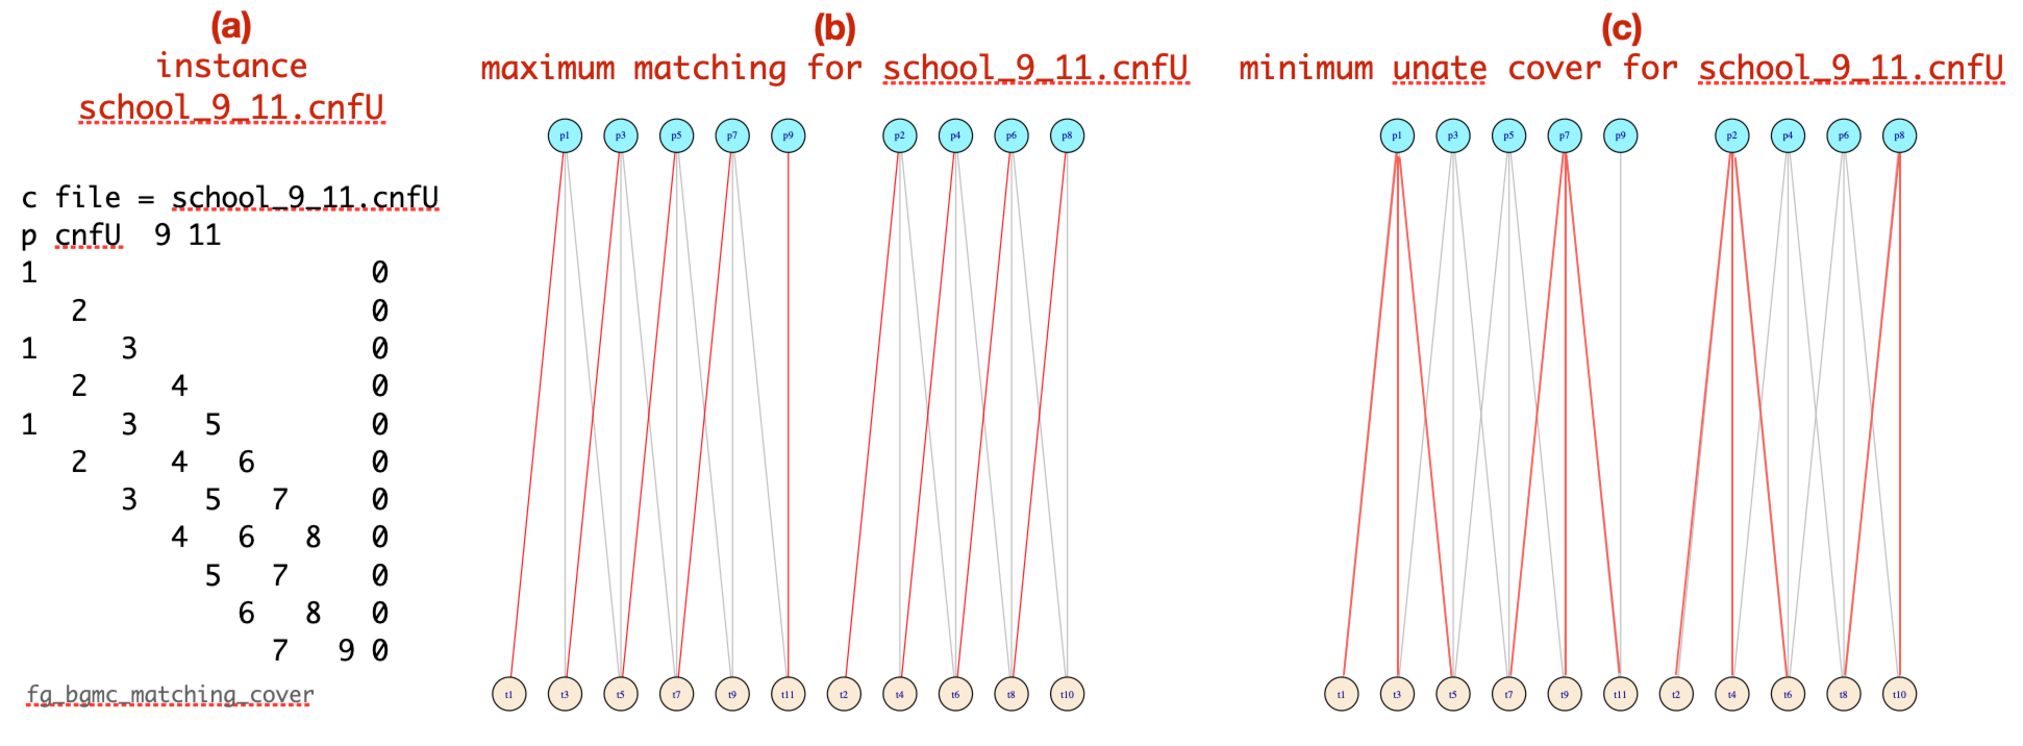
\includegraphics[width=1.00\textwidth]{_Figures/fg_bgmc_matching_cover}

\caption{
Three views of the
instance  {\tt school\_9\_11\_\_0.cnfU} 
introduced in Table~\ref{tb_bgmc_data}: 
{\sf(a)}~
an 11-row, 9-column  sparse matrix 
in a {\it cnf format}~\cite{OPUS-cnf-2021-wiki},
{\sf(b)}~
the maximum bipartite matching problem:
with 9 red edges representing the optimum solution,
{\sf(c)}~
the minimum set covering problem:
4 vertices at the top cover all 11 vertices at the bottom
as illustrated with 11 edges.
}
\label{fg_bgmc_matching_cover}
\end{figure*}


\begin{figure*}[h!]
\vspace*{2ex}
\centering
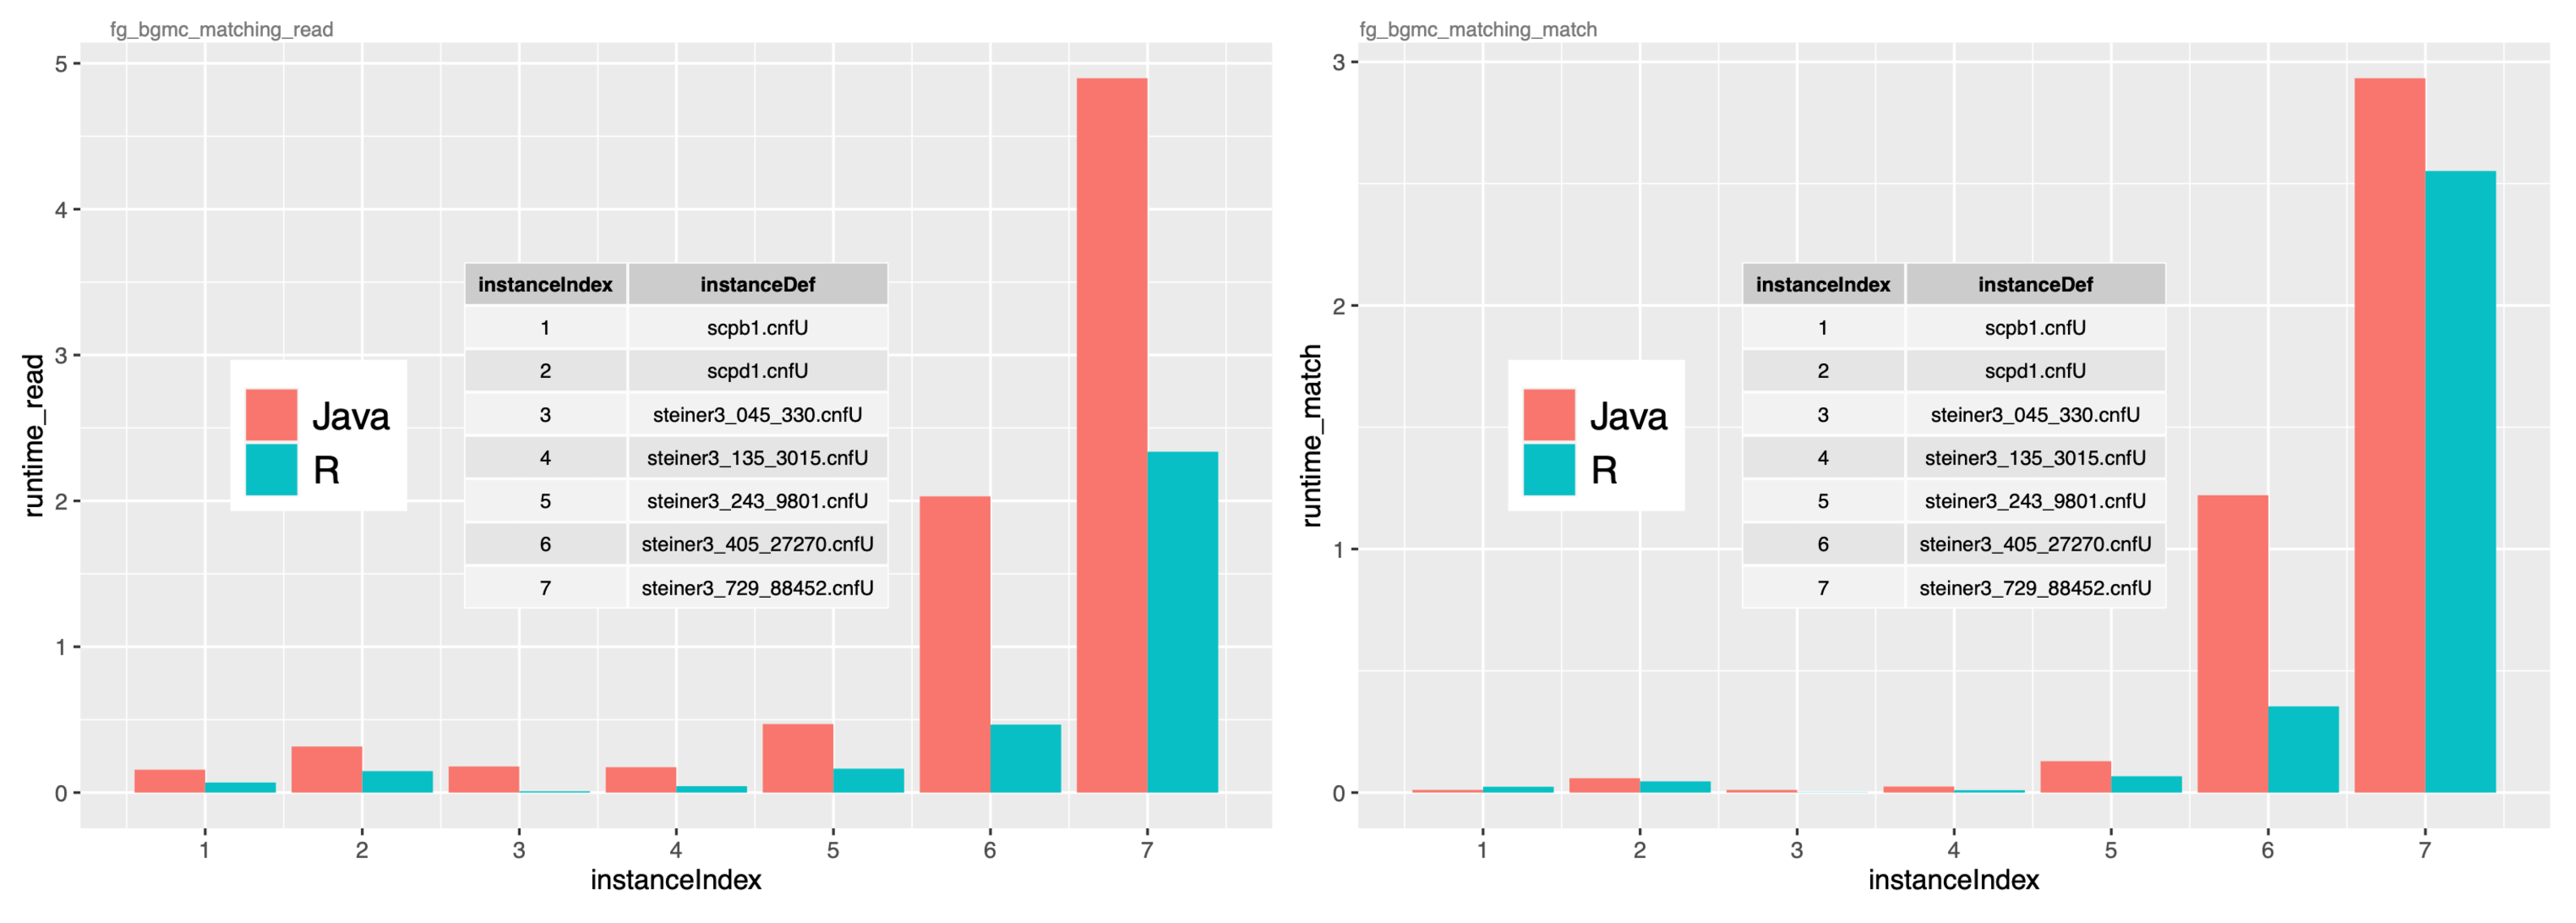
\includegraphics[width=1.00\textwidth]{_Figures/fg_bgmc_matching_experiment}

\caption{
Maximum bipartite matching experiments with three datasets 
steiner3~\cite{OPUS-setc-2021-Resende-steiner3_data}, 
orlib~\cite{OPUS-setc-2014-orlib-Beasley}, 
and random~\cite{OPUS2-1993-benchm-Logic_synthesis}
and two solvers:
the solver in Java~\cite{OPUS-matching-2021-geeksforgeeks-java} and
the solver in \R{}~\cite{OPUS-matching-2021-igraph-R}.
The plot on left
shows the {\tt runtime\_read} for both solvers. 
The plot on right
shows the {\tt runtime\_match} for both solvers, 
i.e. the runtime to find the maximum matching. 
Only instances with runtimes $\ge$ 0.15 seconds are shown.}
\label{fg_bgmc_matching_experiment}
\end{figure*}


The example in Figure~\ref{fg_bgmc_matching_cover} illustrates 
three views of the
instance  {\tt school\_9\_11\_\_0.cnfU} 
introduced in Table~\ref{tb_bgmc_data}: 

\begin{description}

\item[\sf{Figure~\ref{fg_bgmc_matching_cover}a}]~\\\
an 11-row, 9-column  %sparse 
matrix in a {\it cnf format}~\cite{OPUS-cnf-2021-wiki}.


\item[\sf{Figure~\ref{fg_bgmc_matching_cover}b}]~\\\
a bigraph as a two-layered graph 
that illustrates the {\em maximum matching problem}:
11 applicants applying for  1, 2, or 3 of the
9 jobs (teaching positions)  advertised by a school.
Each job opening can only accept one applicant and a 
job applicant can be appointed for only one job. 
In this example, 9 applicants have been matched to 9 jobs:
each match is represented by a red-colored edge.

\item[\sf{Figure~\ref{fg_bgmc_matching_cover}c}]~\\\
a bigraph as a two-layered graph 
illustrates the  {\it a unate covering problem}:
11 subjects (math, physics, etc)  can be taught by 9 instructors.
Seven instructors can teach up to 3 subjects, one instructor can
teach 2 subjects, one instructor can teach 1 subject only.
The objective of the school principal is to hire the minimum
number of teachers while still able to offer classes 
for the 11 subjects. In contrast to the maximum matching problem,
the minimum cost solution for this
covering problem is not as obvious as it is for the matching problem,
even for this small example.
There are only two minimum cost solutions: a total of  4
instructors can teach all subjects. The red-colored edges 
identify 3 instructors who will teach three
subjects and 1 instructor will teach two subjects.

\end{description}

The extension of the unate set cover to the binate set cover
problem requires addition of {\it binate clauses} as
additional rows in the sparse matrix configuration.
For example, if applicants '2' and '5' are a married couple,
and the school principal would like to hire them both,
the matrix in Figure~\ref{fg_bgmc_matching_cover}a 
will be extended with these two rows:
\\[2.5ex]
\hspace*{14ex}{\tt -2 ~~~5}\\
\hspace*{14ex}{\tt ~2 ~~-5}

On the other hand,  if applicants '4' and '7' are a divorced couple,
the school principal may prefer to find a minimum cover solution that
precludes the hiring of these two individuals together: either 
'4' or '7' may be hired but not both. In this case, 
the matrix in Figure~\ref{fg_bgmc_matching_cover}a 
will be extended with this row:
\\[1.5ex]
\hspace*{14ex}{\tt -4 ~~-7}

\subsection{{\sf Runtime experiments: Java vs R}}
\noindent
Our asymptotic experiments have been performed
with two solvers:
one implemented in Java~\cite{OPUS-matching-2021-geeksforgeeks-java}, 
the other implemented in \R{}~\cite{OPUS-matching-2021-igraph-R}.
Both rely on Ford-Fulkerson method~\cite{OPUS-matching-1956-Math-Ford_Fulkerson-max_flows}. The instances tested by both solvers have been introduced in
Table~\ref{tb_bgmc_data}. 
The results are summarized
in Figure~\ref{fg_bgmc_matching_experiment}, but only for instances with runtimes $\ge$ 0.15 seconds.
Most importantly, we separate the total runtime into two components:
(1) runtime to read and set-up all data structures ({\tt runtime\_read}),
(2) runtime to find the maximum matching ({\tt runtime\_match}).

\begin{description}

\item[\sf{runtime\_read}:]~\\\
 Java is significantly outperformed by \R{}.
 For the largest instance steiner3\_729\_88452.cnfU (729 columns, 88452 rows),
 {\tt runtime\_read\_java} $\approx$ 4.9 seconds, 
 {\tt runtime\_read\_R}    $\approx$ 2.3 seconds.
As instance size increases,
 \R{} gains  advantage when using its {\tt data.table} structure.
 In contrast, Java may need to scan each line and convert the data into a matrix.
 

\item[\sf{runtime\_match}:]~\\\
 All except two instances from
 the subset of OR-library instances, scpb1 and scpd1,
 are below the runtime threshold of {\it less than 0.15 seconds}.
 While Java is consistently outperformed by \R{},
 we would need larger instances to assess whether this trend holds.
 So far, the increase in {\tt runtime\_match} is monotonically increasing
 with the decreasing matrix density, both for Java and R.
 For the largest instance, steiner3\_729\_88452.cnfU,  %(729 columns, 88452 rows),
 {\tt runtime\_match\_java} $\approx$ 2.9 seconds while 
 {\tt runtime\_match\_R}    $\approx$ 2.5 seconds.

%
% \verb|numEdges_steiner3_729 =  80000| \\
% \verb|numEdges_scpd1       = 264374|
%\\
%{\bf TO FINISH THIS SUBSECTION WE NEED an extra column}\\
%{\sf  that will report percM where \\
%percM = percentage for nCols matched maximally\\
%e.g. percM\\
%     1.000 for steiner3\_009\\
%     0.998 for steiner3\_015\\
%     etc}
% \\
% \par
% {\sf before completing edits below, we need to introduce the matrix density values (mDens) \\
%matrixDens = round(numEdges/(nCols*mRows), 4) \\
%}
%> nCols=45 ; mRows = 330 ; mDens = 0.07
%> nCols*mRows*mDens
%[1] 1039.5
%> nCols=300 ; mRows = 3000 ; mDens = 0.05
%> nCols*mRows*mDens
%[1] 45000
%> 

%The number of rows is cleary a significant factor in the runtime performance 
%The number of columns for scpb1.cnfU is 3000, but the number of rows is 300. 
%The instance steiner3\_045\_330.cnfU has 330 rows and only 45 columns.
%
%The runtime performance for this instance is statistically equal to %steiner3\_045\_330.cnfU, which also has around 300 rows but only has 45 columns.
 

\OMIT{ 
 Another important observation is how the number of rows affects the runtime performance in maximum matching. By looking at the table~\ref{tb_bgmc_data}, the number of columns for scpb1.cnfU is 3000, but the number of rows is 300. The runtime performance for this instance is statistically equal to steiner3\_045\_330.cnfU, which also has around 300 rows but only has 45 columns. If we compare the runtime performance of scpb1.cnfU with steiner3\_729\_88452.cnfU, which has 88452 rows, the difference is increasing significantly.
}

\end{description}

\OMIT{ 
We test our solvers with asymptotic experiments shown in Table~\ref{tb_bgmc_data}. The difficulty of solving each instance for maximum matching problem is related to the number of columns or number of rows for each instance. Shown in Figure~\ref{fg_bgmc_matching_experiment}, experiments of bipartite graph matching with three datasets, including steiner3, orlib, and random. The left side of the plot depicts the reading runtime for Java and R program. The right side shows the runtime for finding the maximum matching. The plot only contains instances which have more than 0.15 second runtime performance. One important observation is the runtime performance of reading instances for R is much faster than Java with the size of the instance increases. This is because we use data.table library to read in the data, and it has significant advantage when reading a large dataset into a data table. However, Java may need to scan each line and convert the data into a matrix. Another important observation is how the number of rows affects the runtime performance in maximum matching. By looking at the table~\ref{tb_bgmc_data}, the number of columns for scpb1.cnfU is 3000, but the number of rows is 300. The runtime performance for this instance is statistically equal to steiner3\_045\_330.cnfU, which also has around 300 rows but only has 45 columns. If we compare the runtime performance of scpb1.cnfU with steiner3\_729\_88452.cnfU, which has 88452 rows, the difference is increasing significantly.

Therefore, from Figure~\ref{fg_bgmc_matching_experiment}, we can clearly conclude that one of the most important factors that affects the runtime performance is the number of rows in the matrix, or in our fable, the number of subjects that needs to cover. If the number of subjects in the high school is increasing, it would be much harder for the manager to assign maximum number of teachers. With these results, we can also prove that the time complexity stated in the previous section is rational.
}
















